
\documentclass[aps,prl,reprint]{revtex4-2}
\usepackage{gensymb}
\usepackage{graphicx}
\usepackage{amsmath}
\usepackage{hyperref}
\usepackage{dsfont}
\usepackage{relsize}
\usepackage{wrapfig}
\usepackage{graphicx}
\usepackage{hyperref}
\hypersetup{colorlinks=true, citecolor=blue, urlcolor=blue, linkcolor=blue}


\begin{document}

% Use the \preprint command to place your local institutional report
% number in the upper righthand corner of the title page in preprint mode.
% Multiple \preprint commands are allowed.
% Use the 'preprintnumbers' class option to override journal defaults
% to display numbers if necessary
%\preprint{}

%Title of paper
\title{AFT Lab}

% repeat the \author .. \affiliation  etc. as needed
% \email, \thanks, \homepage, \altaffiliation all apply to the current
% author. Explanatory text should go in the []'s, actual e-mail
% address or url should go in the {}'s for \email and \homepage.
% Please use the appropriate macro foreach each type of information

% \affiliation command applies to all authors since the last
% \affiliation command. The \affiliation command should follow the
% other information
% \affiliation can be followed by \email, \homepage, \thanks as well.
\author{Trevor Smith, Alex Storrer}
\email[]{smith.tr@northeastern.edu}
\homepage[]{https://github.com/trevorm4x/}
%\thanks{}
%\altaffiliation{}
\affiliation{Northeastern University}


\date{\today}

\begin{abstract}
	The relationship between both sample rate and number of cycles
	with FFT linewidth was established, and it was found that 
	the number of cycles observed cycles was much more relevant
	in precisely calculating the frequency of a signal.
	It was observed that sampling a signal at a sample rate
	lower than twice that of the signal does not produce
	an accurate reconstruction of the signal in the time
	domain or the frequency domain. Several acoustic sounds
	were produced in the lab and analyzed. It was found that tuning forks
	tuned to the same note will produce an observable acoustic
	``beat" due to their slight differences in frequency. 
	It was found that a human whistle produces only a single,
	pure tone, and the sound produced by two humans whistling 
	the same note is indistinguishable. Several human vowel
	sounds were analyzed, and it was found that each vowel
	sound has a unique frequency signature, and that these
	vowel sounds can be differentiated from each other clearly.
	Finally, two string-based instruments were analyzed for the
	quality of their timbre, or the harmonics present in their
	music. A guitar was found to have much fewer harmonics, and
	lower overall harmonics than a single-string guitar, which
	has much higher harmonics and a great many harmonics.
\end{abstract}


\maketitle

% body of paper here - Use proper section commands
% References should be done using the \cite, \ref, and \label commands
\section{Introduction}
% The Introduction should contain 1 or 2 paragraphs.
% Briefly state the physics underlying the experiment
% (what is being tested and why). 
Fourier analysis is the practice of viewing a time-domain signal in the
frequency domain. Named after the mathemetician Joseph Fourier for his 
breakthrough discovery that most functions, even discontinuous functions
like the step function, can be represented as an infinite sum of sine 
waves, the advancement was originally made in pursuit of more easily
solving complex differential equations describing heat transfer. Some 
scientists and engineers, however, do Fourier wrong by simply
referring to the technique by the anagram of its modern discrete 
implementation, by saying, for example, ``plot the FFT". \\

The FFT, short for Fast-Fourier Transform, is as stated a method for
calculating the discrete Fourier transform of a finite time-domain signal.
One can forgive those who refer to Fourier analysis generally as ``FFT", 
considering how this ingenious algorithm has paved the way for
the discrete Fourier transform's widespread usage in signal processing
across a wide range of fields and disciplines. \\

Utilizing a divide-and-conquer technique, the FFT could be compared to 
a sailboat that, rather than following the wind directly to its destination,
turns sharply to the side and tacks back and forth across the wind,
taking a significantly longer and more complicated path that arrives in 
a fraction of the time. To understand just how well this analogy works,
consider that the first step the FFT performs on a signal of length 2049
is to add another 2047 zeros onto the end so that the signal length is 
an exact power of 2. \\

In this lab we will be conducting Fourier analysis, with the help of the 
FFT algorithm, of various acoustic signals. This analysis is particularly
interesting in the context of speech and musical instruments, as noised that
to our ears may sound like ``one" note or vowel sound are in fact more
often than not rich with multiple harmonics throughout the frequency spectrum.\\

We will first conduct a simplified test implemented entirely in software,
examining the effect of longer observations on the linewidth, or uncertainty
in the frequency domain, numerically. We will then conduct a simple test
using an function generator with an oscilloscope to collect data for a 
sine wave and square wave, in order to compare their frequency responses. \\

In the next phase of the lab, acoustic signals will be examined. 
First, we will explore the interaction of two tuning forks as they 
constructively and destructively interfere due to slight differences 
in their frequency, producing what is known as a ``beat". We will then
explore characteristics of musical notes produced by a whistling sound, 
the human voice producing vowel sounds, and musical instruments. \\

Finally, we will conduct a numerical exploration of the breakdown of accurate
signal reconstruction in the time-domain as a function of the nyquist
frequency and the fundamental frequency of the signal. 

\section{Apparatus}
% List equipment components (manufacturer, model
% numbers and brief specifications). 

The apparatus consisted of the following.
\begin{itemize}
\end{itemize}

\section{Basic FFT}
% Briefly describe the experimental procedures (in your own words, but don’t overdo it)
% Discuss calibrations, etc., if required
% Include necessary equations and put them on their own line (number them, e.g. “Eq. (3)”)
% Include plots showing relevant results (label each figure, e.g. “Fig. 3”, with caption).
% Describe what you found (describe what the plot illustrates)

\subsection{Procedure and Results}

In this section, a time-vector from 0 to 0.1 using 2048 equally spaced points
was produced, and used to build a sine wave of equation $y=sin(2\pi 100 x)$, 
shown in \ref{shortsine_TD}.
The signal was then transformed into the frequency domain, using the 
FFT algorithm. With this signal, as with all signals for the duration of the
lab, the signal was multiplied by a hamming window before performing the
discrete Fourier transform to mitigate spectral leakage. \\


\begin{figure}[h]
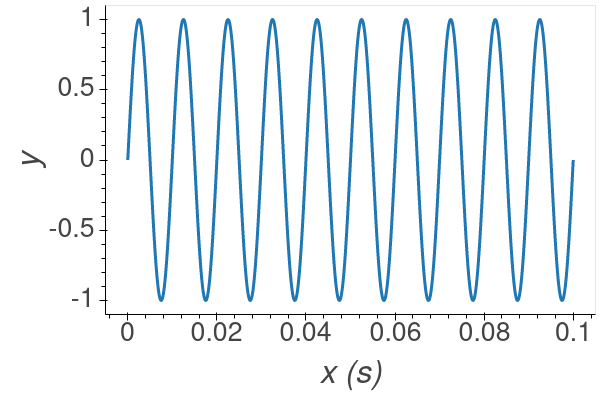
\includegraphics[width=0.34\textwidth]{../Images/l5_A_1a.png}
\caption{\label{shortsine_TD} Sine wave of frequency 100 Hz, observed for 0.1 seconds.}
\end{figure}

The Fourier analysis produced the expected frequency of 100 Hz, verifying that
the technique was applied correctly, as seen in \ref{shortsine_FD}. 

\begin{figure}[h]
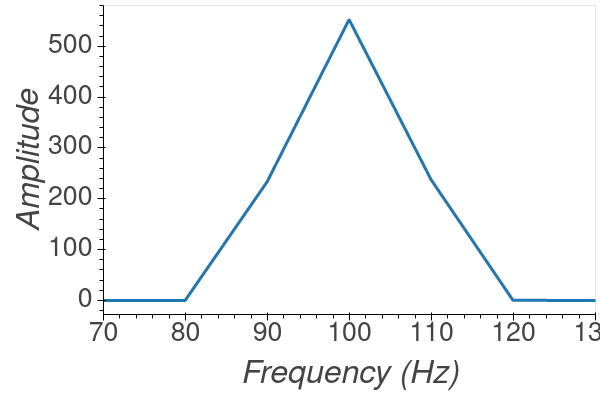
\includegraphics[width=0.34\textwidth]{../Images/l5_A_1b.png}
\caption{\label{shortsine_FD} Sine wave of frequency 100 Hz, observed for 0.1 seconds, in the frequency domain.}
\end{figure}

A second sine signal, calculated with the same sine function and N samples
but longer observation window of 1 second, was produced, as seen in 
\ref{longsine_TD}.

\begin{figure}[h]
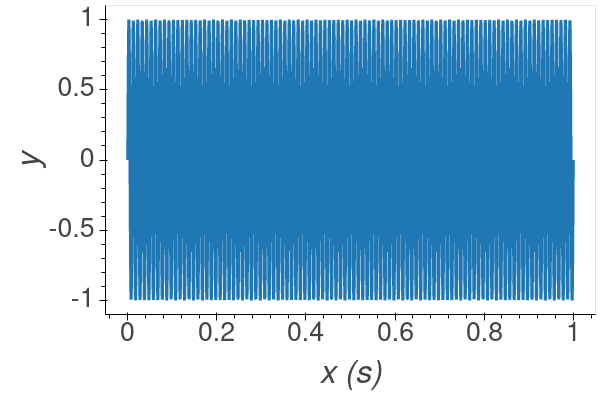
\includegraphics[width=0.34\textwidth]{../Images/l5_A_2a.png}
\caption{\label{shortsine_TD} Sine wave of frequency 100 Hz, observed for 1.0 seconds.}
\end{figure}

This longer sine wave was analyzed in the frequency domain as well, producing
a 100 Hz peak, as seen in \ref{longsine_FD} with the same x-axis range as 
\ref{shortsine_FD}.

\begin{figure}[h]
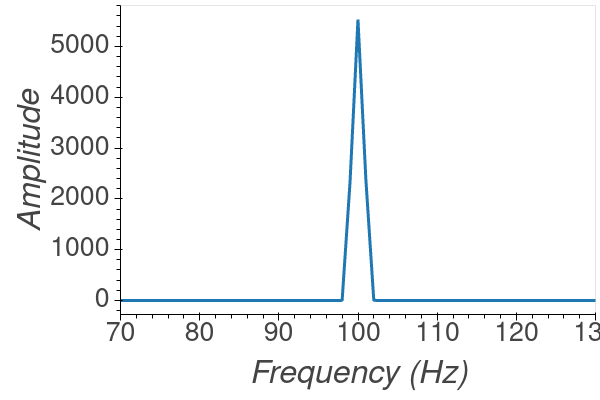
\includegraphics[width=0.34\textwidth]{../Images/l5_A_2b.png}
\caption{\label{shortsine_TD} Sine wave of frequency 100 Hz, observed for 1.0 seconds, in the frequency domain.}
\end{figure}

The characteristics of these two alike signals can be easily compared in 
\ref{comparisine_FD}, however quantitative characteristics are also given in 
\ref{comparisine_TB}. 

\begin{figure}[h]
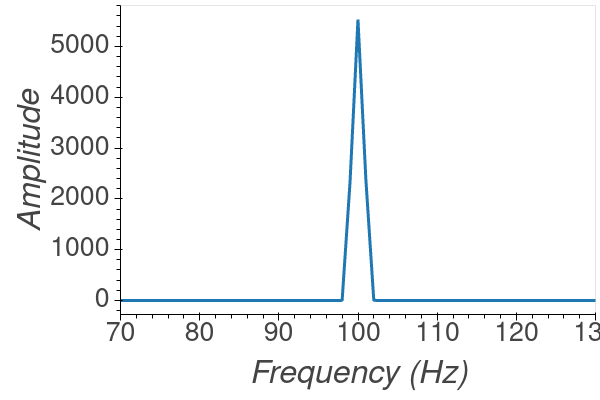
\includegraphics[width=0.34\textwidth]{../Images/l5_A_2b.png}
\caption{\label{comparisine_FD} Comparison of the short (0.1 second) and long
(1.0 second) sine waves, given by the same equation, using Fourier analysis.}
\end{figure}

A brief exploration into the effect of the sample rate on the appearance of
a signal, and its corresponding Nyquist frequency, was conducted numerically.
The same sine wave corresponding to the equation $y=sin(2\pi 100 x)$ was
sampled for 0.1 seconds, using 10 and 100 points. Using an understanding
of the Nyquist frequency, which states that the sample rate must be at least
twice that of the sine wave in order to truthfully reconstruct it, the
lowest number of samples per 0.1 seconds that can truthfully reconstruct the
sine wave was plotted as well, along with one less than that number. These four
waves can be seen in \ref{waves}.

\begin{figure}[h]
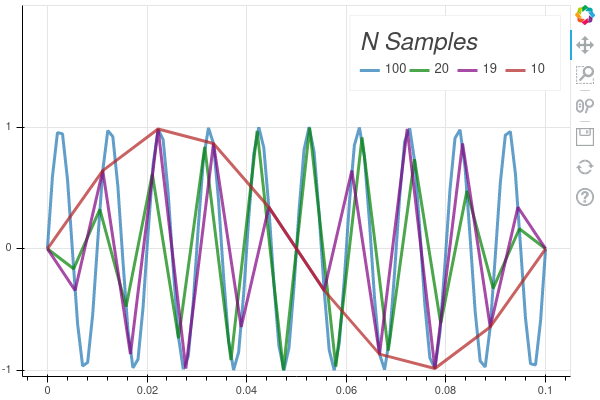
\includegraphics[width=0.44\textwidth]{../Images/l5_optional.png}
\caption{\label{waves} The same equation, sampled with four different numbers
of samples per one tenth of a second.}
\end{figure}

While it is barely visible behind the other curves, it is still clear that
the blue wave is the baseline, a sample rate high enough to reconstruct
the sine wave very well. Because the frequency of the sine wave is 100 Hz,
the lowest Nyquist frequency acceptable would be 200 Hz, or 20 samples over
0.1 seconds. From this it is clear why the red wave, sampled at a rate
such that the Nyquist frequency of that wave is half of what is needed,
does not match the true sine wave whatsoever and looks like a completely
different signal. Observing that this red signal appears to make exactly one
cycle in 0.1 seconds, we can see that it looks like a 10 Hz signal instead of
a 100 Hz signal. It is also easy to make out that the green wave, sampled
at 20 samples per second, contains almost exactly two samples per period or 
one sample per positive and negative peak - the Nyquist frequency corresponding
to that sample rate is exactly the lowest possible value. Finally,
comparing the purple wave, which is sampled with a Nyquist just below the
requisite for this sine wave, to the green and blue waves, it can be seen that
in the middle of the signal it skips a peak, resulting in what looks like a
similar frequency (but slightly lower in frequency) sine wave that is
dampened in the middle. 


\subsection{Conclusion}

Uncertainty in the frequency of a signal, which manifests as the linewidth
of a peak in the frequency domain, is reduced as a function of observation time.
This is the result of a flavor of the Heisenberg Uncertainty Principle, where 
longer observations (greater N cycles) of a signal trade better certainty of 
the location of the signal in the frequency domain for worse certainty of the 
location of the signal in the time domain. \\

This simple experiment confirms that linewidth $\Gamma$ is reduced with
longer observations or more cycles. A higher precision FFT was produced
in this experiment by collecting 100 cycles than by collecting 10 cycles.
It also shows that if a longer observation time is used while the number
N of samples is kept constant, sample rate decreases, which is seen in the
frequency range as well. It is important to note that although the 
resolution of the frequency spectrum was reduced by a factor of ten (larger frequency
bins), the uncertainty or linewidth was still reduced. 

\begin{widetext}
\begin{center}
\begin{table}[t]
\renewcommand{\arraystretch}{1}
\setlength{\tabcolsep}{10pt}
\caption{\label{comparisine_TB} Frequency response and parameters given by a
short and long observation of the same sine equation.}
\begin{tabular}{|c|c|c|c|c|c|}
%\hline
\toprule
Time (s) & Cycles M & Samples N & FFT Range $\Delta f$ & Resolving Power $\frac{f_0}{\delta f}$ (Hz) & Linewidth $\Gamma$ (Hz) \\
\colrule
0.1  &  10   &  2048  &  10225   & 10.00 &  17.4 \\ \colrule
1.0  &  100  &  2048  &  1022.5  & 1.000 &  1.74 \\ \hline
\botrule
\end{tabular}
\end{table}
\end{center}
\end{widetext}

\section{Tuning Forks}

\subsection{Procedure and Results}

In this section, the beat frequency of two tuning forks tuned to the same note
was analyzed. An acoustic ``beat" is caused by a slight difference in the
frequency of two sounds. Because sounds are waves and can constructively or
destructively interfere with each other, two waves of constant frequency can
interact with each other at a fixed point in space with a repeating pattern. 
Specifically, a ``beat" usually occurs when the two constant frequencies are
just slightly different. So, while two tuning forks are more or less exactly
the same to most human ears, the frequency difference between them when they
are played simultaneously may produce an audible ``beat".\\

Two tuning forks were selected, and held at equal distances from a microphone
connected through an amplifier to an oscilloscope. The resulting wave was 
recorded and is shown in \ref{forks}.

\begin{figure}[h]
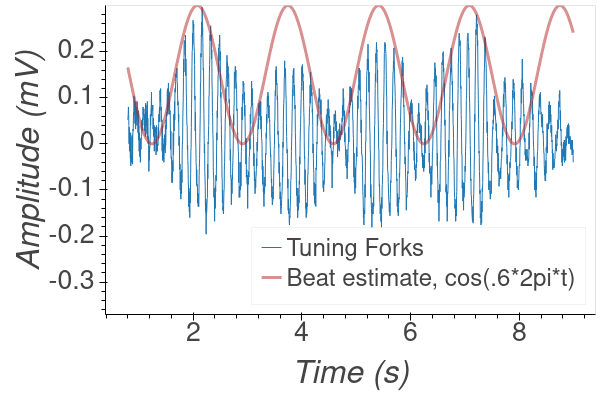
\includegraphics[width=0.44\textwidth]{../Images/l5_C_a.png}
\caption{\label{comparisine_FD} Two tuning forks of nearly equal pitch interacting
in a constructive/destructive pattern, or ``beat", with an estimation of this
beat frequency. }
\end{figure}

The frequency of the tuning forks can be seen as the waves of shorter wavelength,
and the interaction of the two slightly different notes producing a ``beat" can
be seen as the oscillating amplitude of these peaks. It should be noted that
the frequency of the tuning forks themselves may not be accurately represented
at this sample rate, as the nyquist frequency is 120 Hz but the frequency of
the tuning forks is in the thousands. The low sample rate was necessary to observe
the beat pattern, as this was the priority of this experiment. The frequency of these
beats was estimated using trial-and-error at about 0.6 Hz. This fit is not
perfect, perhaps due to holding the forks at inconsitent distances from the
microphone. 

\section{Whistle}

\subsection{Procedure}

In the next phase of the lab, a human whistle was produced by two different
subjects and analyzed in the frequency domain. As in the last section and
in all following sections, the acoustic sounds were recorded with a microphone,
and sampled with an oscilloscope before being saved and analyzed with Fourier
analysis. Each human subject attempted to produce a constant whistling note
during recording.

\subsection{Results}

In the first part of the test only one person whistled a higher-register note.
The frequency signature of this whistle is shown in \ref{high}.

\begin{figure}[h]
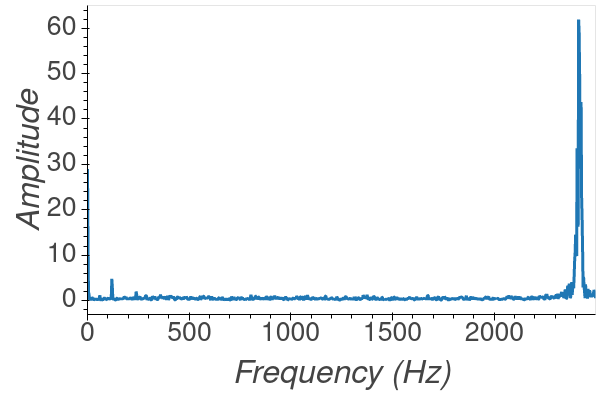
\includegraphics[width=0.44\textwidth]{../Images/l5_D_1.png}
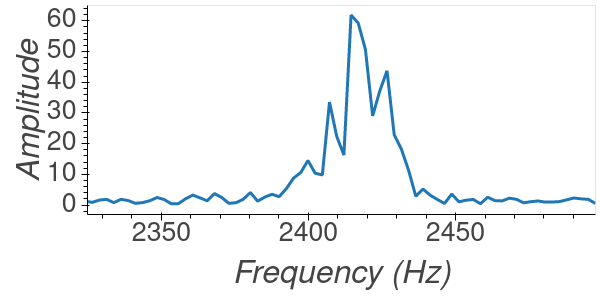
\includegraphics[width=0.44\textwidth]{../Images/l5_D_1_zoomed.png}
\caption{\label{high} The frequency response of a higher-register note
produced by a human whistling, at full scale and zoomed in to the relevant area.}
\end{figure}

Only a single frequency is observed in a human whistle, similar to what may
be expected from a tuning fork. While it is true that the zoomed in version
of the FFT in \ref{high} reveals a non-zero linewidth and seems to include a few
frequency components, this is likely due to the subject's whistling skill
being inhibited by wearing a face-mask, causing the note to waver in pitch 
slightly. \\

\newpage

In the next part of this test, two subjects, Adrian and Trevor,
whistled the same note, recording
them separately. A lower note was used that was within both subjects' registers.
This is shown in \ref{low}.

\begin{figure}[h]
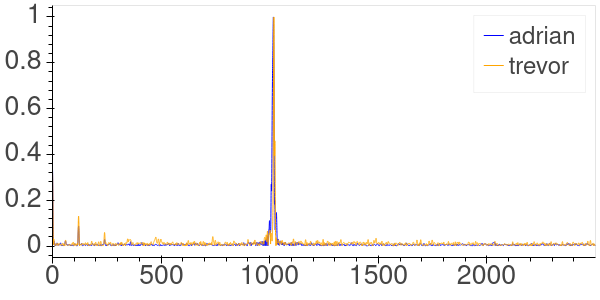
\includegraphics[width=0.44\textwidth]{../Images/l5_D_2.png}
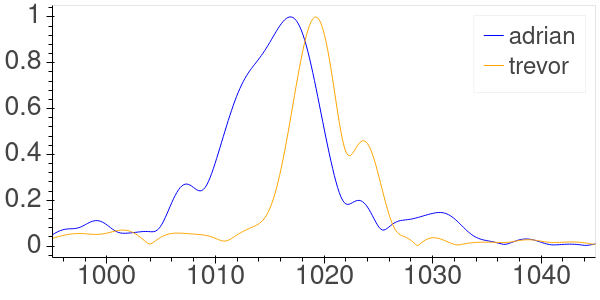
\includegraphics[width=0.44\textwidth]{../Images/l5_D_2_zoomed.png}
\caption{\label{low} The normalized frequency response of
two subjects recording the same whistling note separately.}
\end{figure}

Again, as before, a single frequency was observed for both subjects' 
whistles. While a zoomed in view does seem to show that Adrian's whistle
involves slightly more variation lower than the main note, this is likely
simply a matter of Adrian not holding the exact same note during testing,
while Trevor's note was more consistent. For both whistlers, there are 
no harmonics present in the Fourier analysis. 

\subsection{Conclusion}

It appears for all intents and purposes that the whistle of one identical,
constant note by two people are indistinguishable. This is indicative
of the physiology of whistling. \\

In order to produce a whistle, there is at the core an interaction between
high-speed air and still air that forms a ``vortex ring". This occurs 
in the space between the tongue, pushed up against the roof of the mouth,
and the lips, inside the mouth. As these rings of circulating air hit the
lips, a pressure wave is sent back into the mouth. A whistler is able
to shape their mouth such that this pressure wave resonates with the 
formation of new vortex rings. \\

It is this mechanism that amplifies the overall sound and produces a single,
pure tone. This is because there is only one path that the sound travels,
and nodes only at the back of the tongue and the lips. \\

It is true, though, that just because the same note held by two people is
indistinguishable, doesn't mean that all whistling is the same. Because
whistling is a musical instrument, artistic talent is required to produce 
music, and this artistic talent may be observable from one person to the next.

\section{Human Voice}

\subsection{Procedure and Results}

In this phase of the lab, several vowel sounds were produced, recorded with
a microphone and oscilloscope, and analyzed in the frequency domain. These
vowel sounds were `a', `e', `o', and `u', pronounced like in `car' with
a bostonian accent, `cheese', `coo coo ca choo', and `choose'. These
sounds were produced by a human male with a relatively low voice. The frequency
response of these 5 vowel sounds are shown in \ref{vowels}.


\begin{figure}[h]
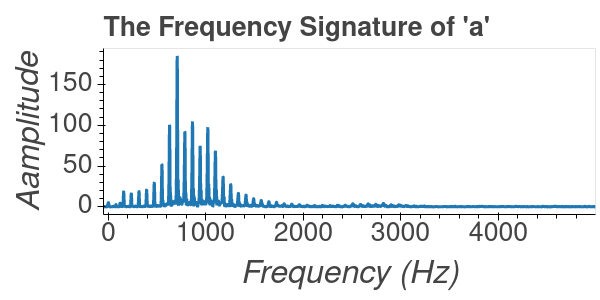
\includegraphics[width=0.44\textwidth]{../Images/l5_E_a.png}
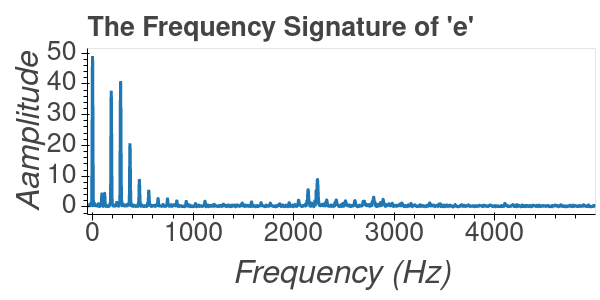
\includegraphics[width=0.44\textwidth]{../Images/l5_E_e.png}
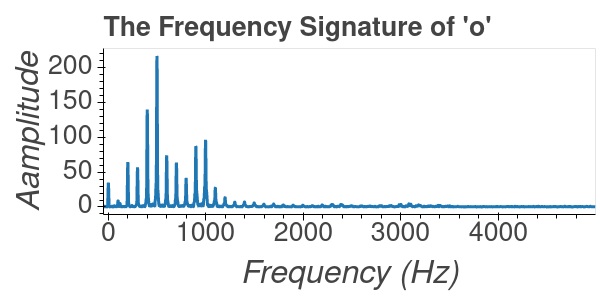
\includegraphics[width=0.44\textwidth]{../Images/l5_E_o.png}
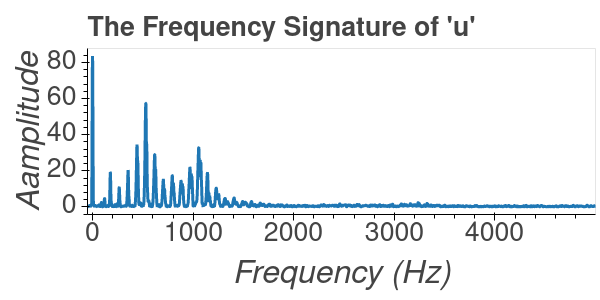
\includegraphics[width=0.44\textwidth]{../Images/l5_E_u.png}
\caption{\label{vowles} The frequency signatures of various vowel sounds.}
\end{figure}

\subsection{Conclusion}

These frequency responses help describe the sounds we are used to hearing
and making in a few ways. \\

First, beginning at the earliest peak, the `0' frequence or offset.
There is a significant peak observed for `e'
and `u', and a small one for `o', but not for `a'. The reason for this is
that for `e' and `u', the sounds are produced by building up pressure at
the very back of the throat and then releasing, while the `a' sound is
simply released without any effort. This pressure wave is recorded as an 
average amplitude greater than zero. Trying to make an `e' sound without
building up pressure feels very awkward. \\

Next, we can look at the number of peaks present. `a', has the most activity
in the frequency domain when judged by number of peaks. This relates to 
the way this sound is produced with an open mouth, with very many different
paths and harmonics available for the sound to be shaped by. `e' has very
vew peaks, which relates to the more closed position of the mouth and the
flat shape of the tongue. `o' and `u' have almost the exact same number of 
peaks and frequencies of said peaks, which relates to them being essentially
the same sound but with a slight shift at the front of the mouth. This shift
serves to shift the relative amplitude of the higher harmonics closer to 
the lower ones. \\

Next, we can look at the locations of the peaks. Perhaps the most interesting
vowel in this regard is `e'. `e' has both the lowest peak frequency and the 
largest higher frequency in the 2 kHz range. This relates to the dropped jaw
leaving more room for the vocal cord to oscillate at a lower frequency, and 
also to the higher pitch resonance created in the nasal cavities. `a' has
a peak frequency that is higher pitched, but has lower and higher amplitude
harmonics, but has very little resonance in the nasal cavities producing
higher frequency harmonics. This can be observed by saying `e' and `a' with
one's nose plugged - the `e' sounds much different but the `a' sounds the
same. Finally, for `o' and `u', the fundamental frequency is much more 
noticable as they are lower-sounding notes, but very many higher sounds
are present, kind of the same sound that is the main one you hear when
humming. 


\section{Musical Harmonics}

\subsection{Procedure and Results}

Finally, the same recording setup as before was used to record two musical
instruments playing the same note. The two selections were a classical
guitar and a single-string. The frequency response of both of these 
instruments playing a C# can be seen in \ref{instruments_ffts}.

\begin{figure}[h]
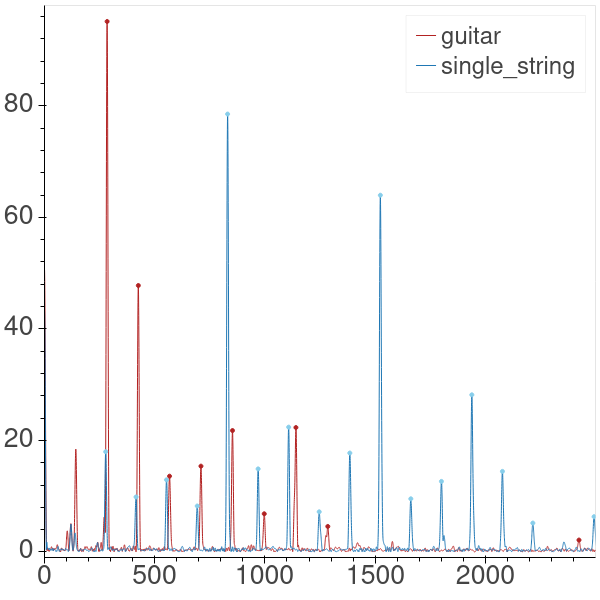
\includegraphics[width=0.44\textwidth]{../Images/l5_f_extra.png}
\caption{\label{instruments_ffts} The frequency response of the two
selected instruments. The locations of peaks used in further analysis
are marked with dots. }
\end{figure}

It is clear that these instruments are indeed quite different from their
frequency response. Most prominent is the comparison between the most
prominent peaks. The guitar's strongest harmonic is very low, the second
harmonic. This makes sense given the construction of the instrument -
there is a very large, hollow body situated just under the location
where one strums, which serves to amplify lower frequencies and increase
the richness of the sound. The single-string's strongest harmonic is much
higher, the fifth harmonic. This makes sense given its construction is just
a single string drilled into a 1/2x3 plank of wood. There is nothing to 
amplify the lower frequencies, and the result is a much tinnier sound. \\

The further point of comparison between the two instruments is the 
amount of harmonics. The guitar has a strong second harmonic (and the
fundamental frequency is also observable), as well four or five more,
much quieter higher harmonics. The single-string has a second, very
significant harmonic at 1500 kHz, and another one at 2000 kHz. This
is much higher than any of the harmonics with a significant amplitude
for the guitar had. In addition, there are just a slew of harmonics,
there's something present at essentially every single harmonic all
the way up to 3000 kHz. \\

To clarify, all musical notes have a single fundamental frequency, the
lowest frequency, and a series of harmonics which are integer multiples
of the fundamental. It is doubtful that any musical instrument 
intentionally has more than one fundamental, as it would sound like
playing two discordant notes at the same time. \\

A summary of the above FFT plot can be seen in \ref{harmonics}, where
each frequency was divided by the fundamental in order to find the
integer factor, or the harmonic number. Each harmonic was also
converted to a musical note. 

\begin{figure}[h]
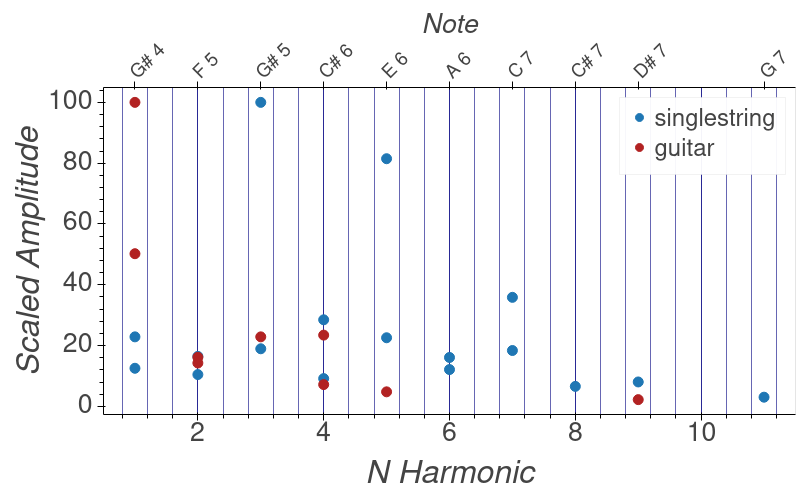
\includegraphics[width=0.44\textwidth]{../Images/l5_f.png}
\caption{\label{harmonics} Normalized plot of the harmonics
of both instruments and their relative amplitudes. }
\end{figure}

This plot clarifies the difference between the two instruments. The
beauty of the guitar as a musical instrument is really striking,
with the C#, the fundamental frequency, harmonizing with a C#
one octave up, a G# which is the fifth half-step below the C#,
and again with another G# and C# in even higher registers. 
For the single-string, by contrast,
while the tuner appropriately picked up the lowest
note, the C# to tune to, the most predominant notes are the 
B and G, where the B is a very awkward two half-steps below
the C#, and the G is a very awkward 6 half-steps below the C#. 
This explains why no matter how tuned it was, the single-string
always sounded out of tune and discordant. \\

For the purpose of demonstration, a long cardboard tube was
used to create a flute-like instrument by cutting a hole near
one end and rounding it with tape. A note was successfully
produced with great effort, which was recorded using a laptop
microphone and saved as an mp3. The A(N) is shown in \ref{flute?}.

\begin{figure}[h]
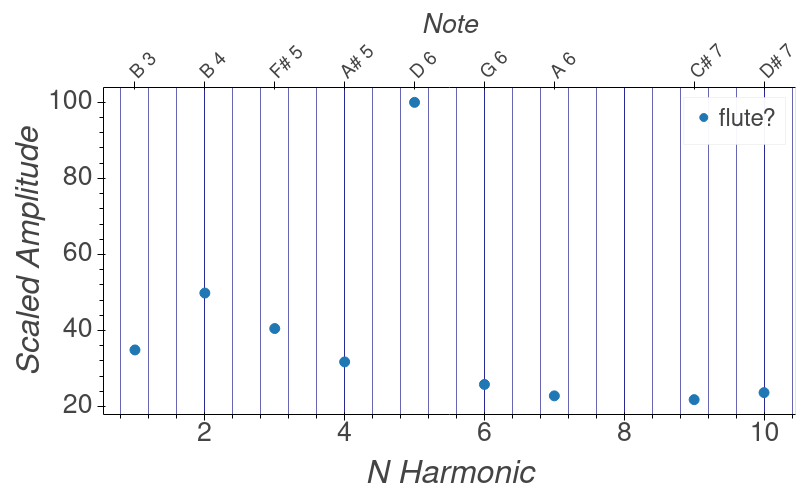
\includegraphics[width=0.44\textwidth]{../Images/l5_optional_flute_harmonics.png}
\caption{\label{flute?} Normalized plot of the harmonics
of a makeshift flute and their relative amplitudes. }
\end{figure}

\begin{figure}[h]
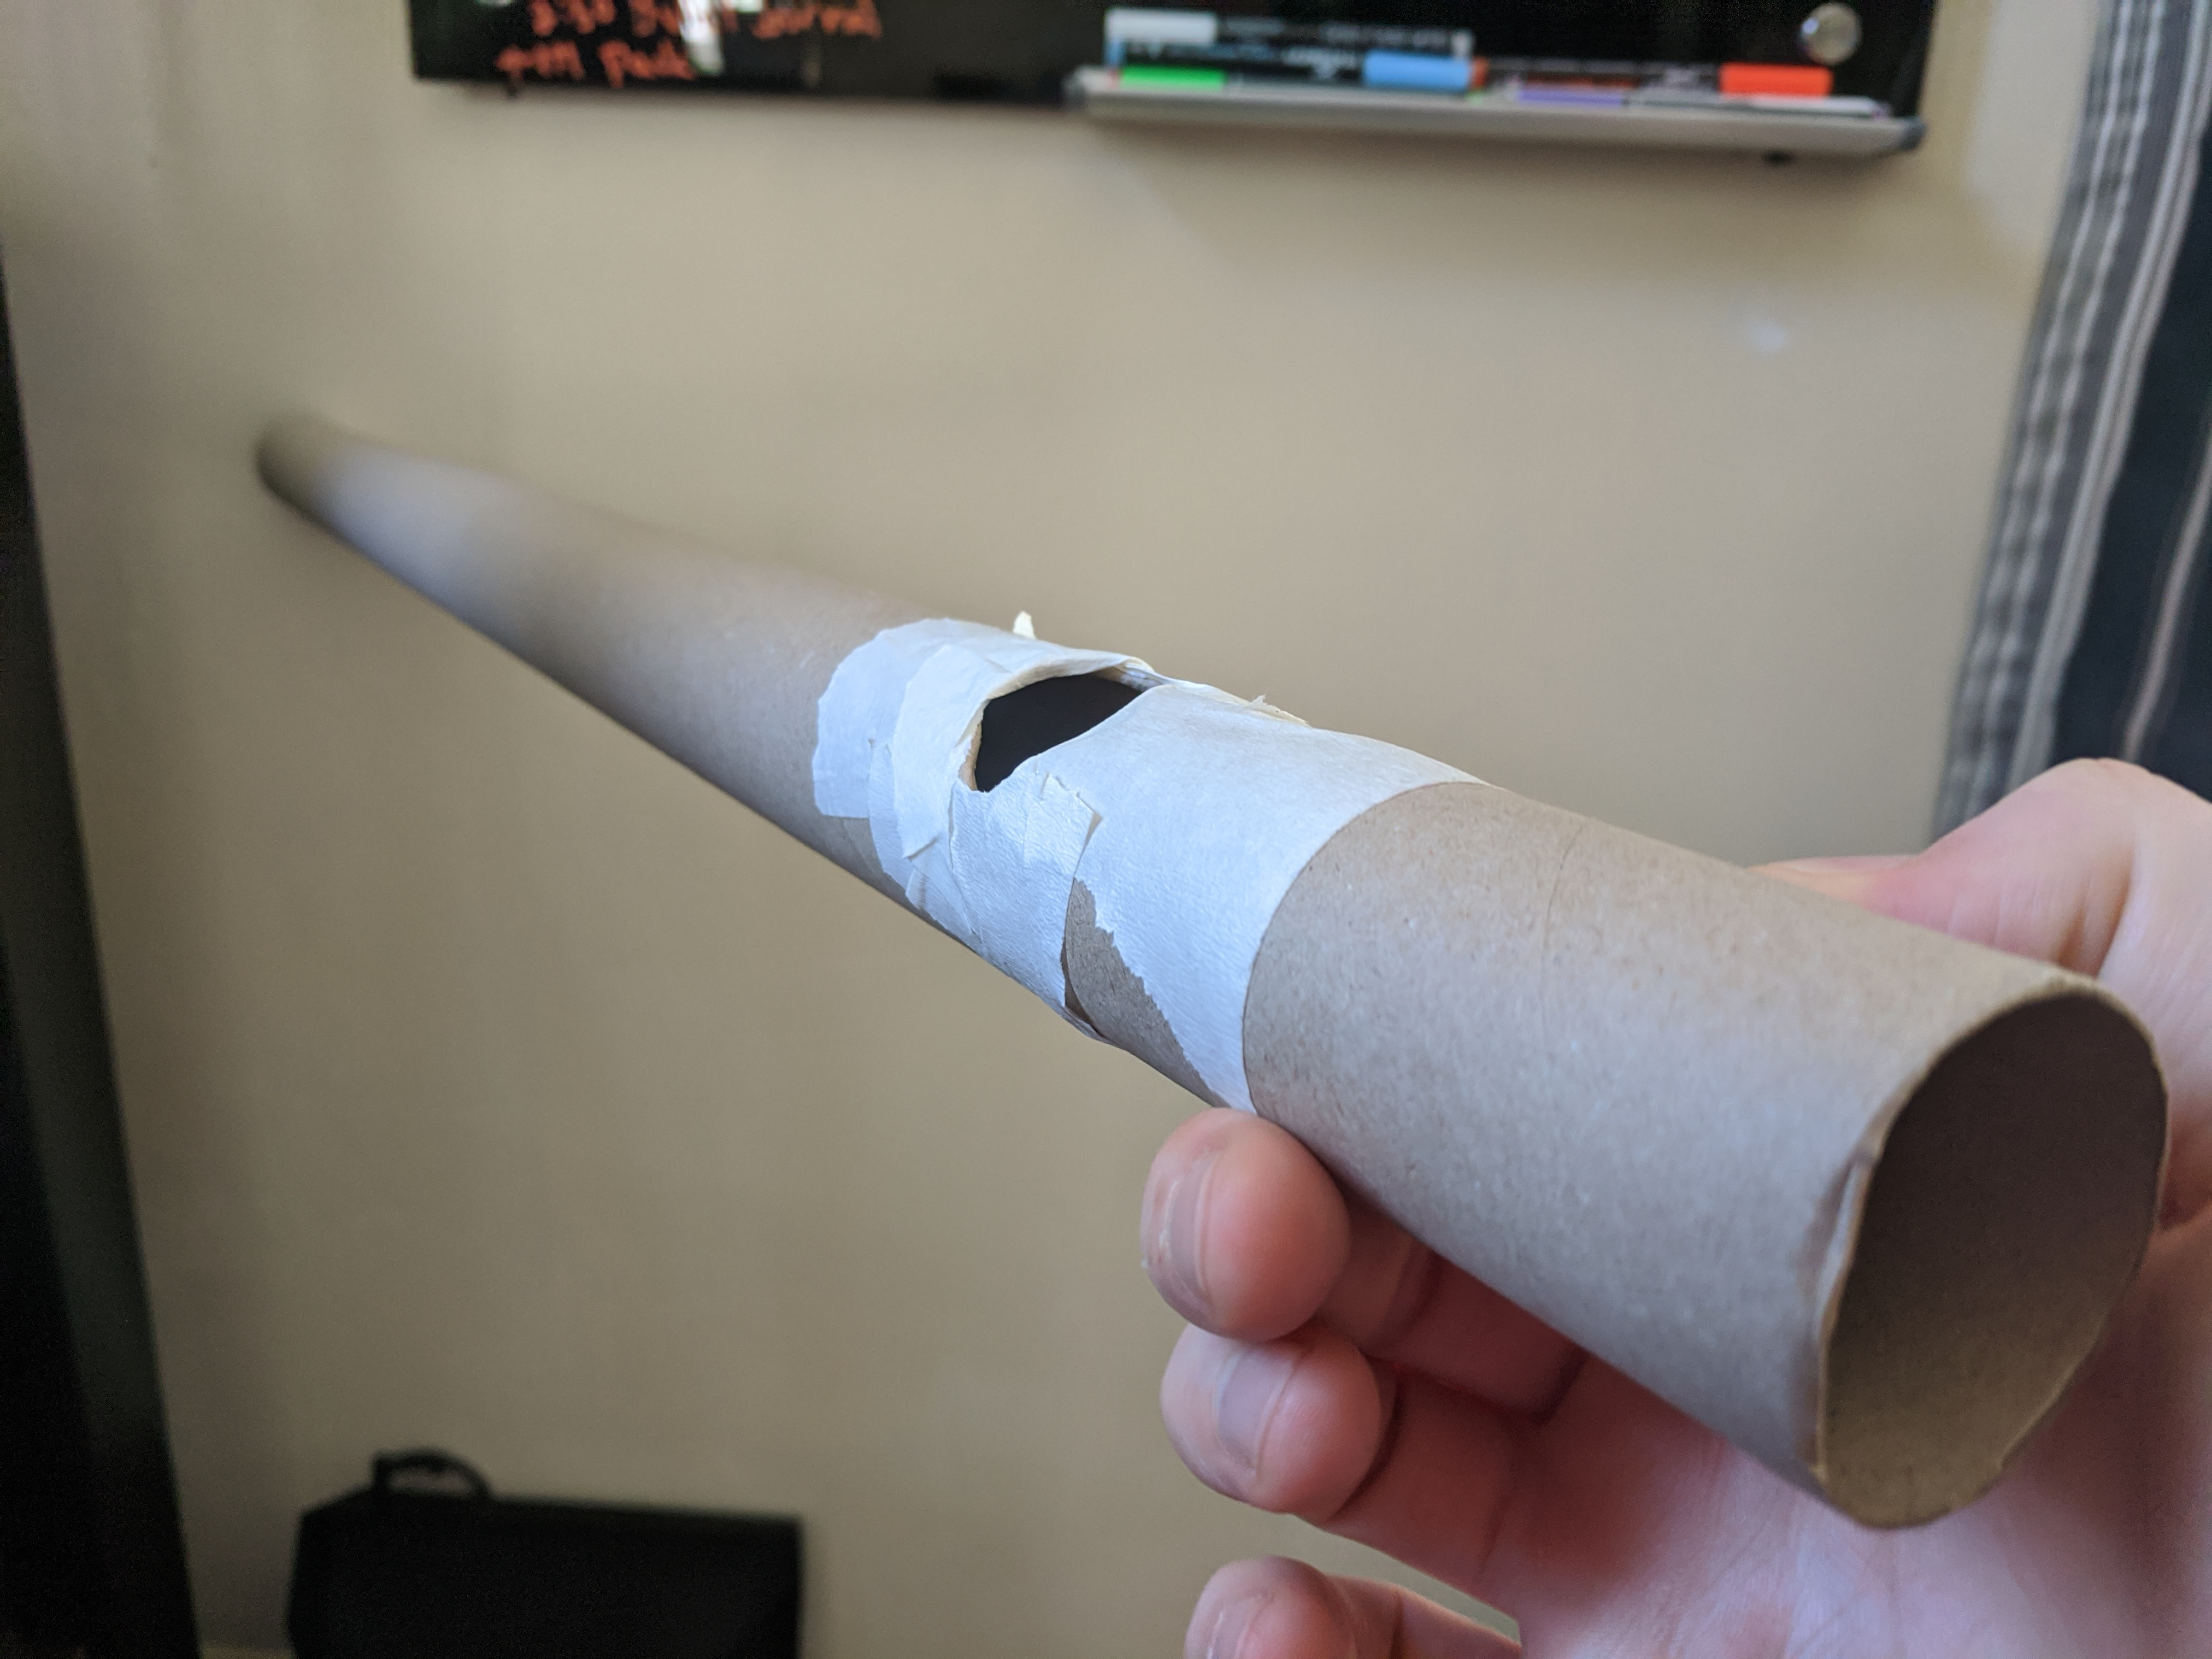
\includegraphics[width=0.44\textwidth]{../Images/l5_optional_flute.jpg}
\caption{\label{flute} Picture of the makeshift flute. }
\end{figure}

It is not clear from seeing the normalized scale, but only one of
these notes was audible, the fifth harmonic. The sound of air
rushing past did seem to produce measurable frequencies which
did correspond to harmonics of a fundamental (corresponding
to the length of the tube), but in reality these other harmonics
just sounded like air blowing through a cardboard tube. It is
unexpected that the main note is the fifth harmonic because
the hole was located about one seventh of the way down the tube,
not one fifth. From this it seems like the point of the tube
where the note was produced was inside the tube. This perhaps
could help design improvements, as the length could be cut down
to match this length of five times the distance from the hole
to the first end. An image is shown in \ref{flute}.



\section{Summary}

The characteristics of several acoustic signals,
and the inherent constraints of Fourier analysis as it pertains
to sample rate, Nyquist frequency, and spectral leakage, were
explored. It was observed that a signal sampled at too
low a sample rate will alias into the lower frequency ranges,
making the signal look like a lower frequency signal. 
It was also observed that, as long as the Nyquist frequency
corresponding to the sample rate is still high enough
to observe the signal, more sine wave cycles is more
important than more samples per second in determining
frequency with very high certainty, or low linewidth. \\

Several acoustic noises were analyzed, and their frequency-
domain characteristics were linked to the character of the
sound that can be observed through listening.
Two tuning forks were struck simultaneously, in order to 
observe the slight difference in their exact tuning through
the pattern of constructive and destructive interference
that it causes, known as acoustic ``beat". This beat was
observed with a period of about 0.6 seconds. \\

A human whistle was analyzed, and it was found to be very
similar in the frequency domain to a single sine wave.
Two subjects produced a whistle at the same note, and
these whistles were sound to be more or less identical.
This was linked to the physiological way that whistles
are produced by humans, which inherently produces only
a single oscillating pressure wave with no harmonics. \\

Several vowel sounds were found to be distinguishable through
a series of frequency-domain features, including a plosive
sound formed by releasing pressure to create the sound,
nasal harmonics, numbers of peaks, and the frequency 
of the highest peak. \\

Several musical instruments were analyzed, two of which
both create sound using strings and were playing the same
note at time of recording, and their timbre was revealed
through Fourier analysis, explaining the rich and deep sound
of the guitar and the tinny and discordant sound of the
single-string. \\

Fourier analysis is truly an insightful tool in the
realm of acoustic physics, and it was all enabled
by Fourier, and the incredible algorithm known as 
the Fast-Fourier-Transform. 






\begin{thebibliography}{9}
\bibitem{fft} 
Wikipedia, Fast Fourier Transform: \\
\href{https://en.wikipedia.org/wiki/Fast_Fourier_transform#History}{https://en.wikipedia.org/wiki/FastFouriertransform}


\bibitem{whistling} 
Wall Street Journal, The Secret of Whistling \\
\href{https://www.wsj.com/?mod=wsjheader_logo}{https://www.wsj.com/?mod=wsjheader_logo}


\bibitem{speech} 
Royal Society Publishing, Bioacoustics of Human Speech \\
\href{https://royalsocietypublishing.org/doi/10.1098/rspb.2019.1116}{https://royalsocietypublishing.org/doi/10.1098/rspb.2019.1116}
\end{thebibliography}


\end{document}
%
% ****** End of file apstemplate.tex ******

